\chapter{Tecnologie e scelte progettuali}
\label{chap:tecnologie-strumenti}

\section{Il problema e le sfide tecnologiche}
\label{sec:problematiche-tecnologiche}
\noindent Affinché il prodotto finale risulti efficace ed effettivamente utilizzabile in scenari reali, è stato necessario tenere in considerazione diverse sfide tecnologiche e architetturali. \newline
In primo luogo l'applicazione deve garantire fluidità e responsività su diversi sistemi operativi (Android e iOS), richiedendo una base di codice manutenibile e scalabile. In secondo luogo, il sistema deve potersi interfacciare in modo sicuro e affidabile con il gestionale \gls{erp} preesistente in Ergon, permettendo l'automazione di diversi processi amministrativi correlati. \newline
Inoltre, il progetto richiede di risolvere due problematiche tecniche di notevole importanza:
\begin{itemize}
    \item \textbf{Funzionamento disconnesso (Offline):} i dipendenti in trasferta potrebbero aver bisogno di registrare una spesa in luoghi privi di connessione a internet. Il sistema deve quindi prevedere un'architettura in grado di salvare i dati localmente per poi sincronizzarli con i server aziendali in un secondo momento.
    \item \textbf{Estrazione automatica dei dati:} per velocizzare l'inserimento, il sistema deve interfacciarsi con l'hardware del dispositivo (la fotocamera) e comunicare con un servizio cloud di \gls{ia} per l'analisi e l'estrazione del testo dai giustificativi cartacei tramite algoritmi di \gls{ocrg}.
\end{itemize}
La risoluzione di queste problematiche ha richiesto un'attenta analisi dello stato dell'arte delle tecnologie attuali, portando alle scelte progettuali descritte nei paragrafi successivi.


\section{Tecnologie per lo sviluppo mobile}
\label{sec:tecnologie-sviluppo-mobile}

\subsection*{Paradigmi di sviluppo mobile}
\label{subsec:stato-arte-mobile}
\noindent Al giorno d'oggi, lo sviluppo di un'applicazione mobile può essere affrontato seguendo tre paradigmi principali, ciascuno con specifici vantaggi e svantaggi in termini di prestazioni, tempi di sviluppo e costi di manutenzione:
\begin{itemize}
    \item \textbf{Sviluppo Nativo:} prevede l'utilizzo di linguaggi e strumenti forniti ufficialmente dai creatori dei sistemi operativi, come Swift per iOS e Kotlin per Android. Questo approccio offre le migliori prestazioni possibili e un accesso diretto alle funzionalità del dispositivo, ma richiede la scrittura di due basi di codice completamente distinte, raddoppiando di fatto i costi e i tempi di sviluppo.
    \item \textbf{Sviluppo Ibrido:} combina elementi di sviluppo nativo e web, utilizzando tecnologie come \textit{HTML}, \textit{CSS} e \textit{JavaScript} per creare applicazioni che possono essere distribuite su più piattaforme. Questo approccio consente di ridurre i costi e i tempi di sviluppo, ma può comportare un compromesso sulle prestazioni grafiche e computazionali rispetto a un'app nativa.
    \item \textbf{Sviluppo Cross-Platform:} prevede l'utilizzo di framework che consentono di scrivere il codice una volta sola e distribuirlo su diverse piattaforme. Questo approccio consente di ottenere prestazioni generalmente vicine a quelle delle applicazioni native, riducendo al contempo i costi di sviluppo e manutenzione.
\end{itemize}

\subsection*{La scelta di .NET MAUI e C\#}
\label{subsec:scelta-maui}
\begin{figure}[H]
    \vspace{2em}
    \centering
    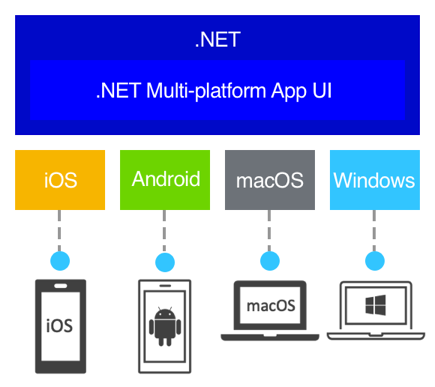
\includegraphics[alt={.NET MAUI}, width=0.75\columnwidth]{img/maui.jpg}
    \caption{.NET MAUI}
    \label{fig:maui}
\end{figure}
\noindent Considerati i requisiti del progetto e la necessità di mantenere coerenza con le tecnologie già adottate in azienda, l'approccio cross-platform è risultato il compromesso più adeguato tra produttività, manutenibilità e prestazioni. Per questo motivo, è stato utilizzato il framework \gls{dotnetmauig}. \newline
Esso rappresenta la naturale evoluzione del framework \textit{Xamarin.Forms} ed è uno strumento open-source fornito da Microsoft che permette di sviluppare applicazioni cross-platform che vengono eseguite utilizzando controlli nativi delle piattaforme target. La logica di business dell'applicazione è scritta interamente in \gls{csharpg} \cite{site:csharp}, un linguaggio di programmazione multi-paradigma e orientato agli oggetti, noto per la sua robustezza e forte tipizzazione. \newline
La scelta di questa tecnologia, in accordo con gli standard aziendali di Ergon, è stata dettata dai seguenti fattori determinanti:
\begin{itemize}
    \item \textbf{Unificazione del linguaggio:} l'\gls{erp} e i web services aziendali di Ergon sono storicamente sviluppati utilizzando l'ecosistema Microsoft e il linguaggio \gls{csharpg}. Utilizzare MAUI ha permesso di mantenere una coerenza tecnologica tra frontend e backend.
    \item \textbf{Produttività e UI condivisa:} MAUI permette di definire l'interfaccia utente in un unico posto utilizzando il linguaggio \gls{xamlg} \cite{site:xaml}. Il framework si occupa poi di tradurre i componenti nei rispettivi controlli nativi di Android o iOS, garantendo all'utente un'esperienza familiare e coerente.
    \item \textbf{Supporto nativo al pattern MVVM:} MAUI è progettato per supportare nativamente il pattern architetturale \gls{mvvm}, che consente di separare in modo chiaro la logica di presentazione dalla logica di business, facilitando il testing e la manutenzione del codice.
\end{itemize}




\section{Persistenza locale e sincronizzazione offline}
\label{sec:persistenza-sincronizzazione}

\subsection*{Database locali nelle applicazioni mobile}
\label{subsec:database-locali}
\noindent Per garantire il funzionamento dell'applicazione anche in assenza di connettività, è necessario adottare una soluzione di persistenza locale che consenta di memorizzare temporaneamente le informazioni direttamente sul dispositivo. Esistono diverse strategie per la memorizzazione locale dei dati nelle applicazioni mobile:
\begin{itemize}
    \item \textbf{File System:} consiste nel salvare i dati all'interno di file, ad esempio in formato \textit{JSON} o \textit{XML}. Questa soluzione è semplice da implementare, ma può diventare difficile da gestire quando il volume dei dati aumenta o quando è necessario effettuare ricerche e aggiornamenti frequenti.
    \item \textbf{Shared Preferences/User Defaults:} si tratta di meccanismi pensati per la memorizzazione di piccoli dati di configurazione o preferenze dell'utente. Sono adatti per dati di piccole dimensioni, ma non per la gestione di informazioni strutturate e persistenti come le note spesa.
    \item \textbf{Database locali:} prevedono l'utilizzo di un database \gls{embeddedg} direttamente sul dispositivo. Questo approccio consente di organizzare i dati in modo strutturato, effettuare interrogazioni efficienti e garantire una maggiore affidabilità nella gestione delle informazioni.
\end{itemize}

\subsection*{La scelta di SQLite}
\label{subsec:sqlite}
\begin{figure}[H]
    \vspace{2em}
    \centering
    
\includegraphics[alt={SQLite}, width=0.40\columnwidth]{img/sqlite.jpg}
    \caption{Logo di SQLite}
    \label{fig:sqlite}
\end{figure}

\noindent Per la gestione della persistenza locale è stato scelto \gls{sqliteg} \cite{site:sqlite} , un database relazionale embedded ampiamente utilizzato nello sviluppo mobile. La scelta è motivata da diversi fattori:
\begin{itemize}
    \item \textbf{Organizzazione strutturata dei dati:} \gls{sqliteg} permette di memorizzare le informazioni all'interno di tabelle relazionali, facilitando la gestione delle note spesa e delle relative informazioni associate.
    \item \textbf{Leggerezza e affidabilità:} il database è progettato per funzionare direttamente sul dispositivo senza richiedere componenti server aggiuntivi, risultando leggero e affidabile anche in condizioni di risorse limitate come nel caso di dispositivi mobili.
    \item \textbf{Integrazione con l'ecosistema .NET:} \gls{sqliteg} dispone di librerie mature e ben supportate per \gls{dotnetmauig}, consentendo una gestione semplice delle operazioni di lettura e scrittura dei dati.
\end{itemize}
Grazie a questa soluzione, l'applicazione è in grado di salvare localmente le note spesa create dall'utente anche in assenza di connessione Internet. Una volta ristabilita la connettività, l'utente può sincronizzare i dati con i servizi esposti dal sistema aziendale tramite chiamate \gls{apirestg}, garantendo così la coerenza delle informazioni tra dispositivo mobile ed \gls{erp}.


\section{Elaborazione automatica delle immagini}
\label{sec:elaborazione-immagini}

\subsection*{La tecnologia OCR}
\label{subsec:teoria-ocr}
\noindent L'elaborazione delle immagini per l'estrazione del testo si basa sulla tecnologia \gls{ocr}, la quale permette di rilevare e tradurre i caratteri presenti all'interno di un'immagine digitale o di un documento scansionato in testo che può essere elaborato e interpretato da una macchina. 
Il processo di riconoscimento ottico dei caratteri prevede generalmente diverse fasi sequenziali: 
\begin{itemize}
    \item acquisizione dell'immagine;
    \item pre-processamento per migliorarne la qualità;
    \item segmentazione per isolare i blocchi di testo e i singoli caratteri;
    \item riconoscimento vero e proprio tramite algoritmi complessi.
\end{itemize} 
L'adozione di questa tecnologia nel progetto è fondamentale per digitalizzare rapidamente documenti cartacei come gli scontrini, riducendo drasticamente i tempi di inserimento manuale da parte dell'utente e minimizzando i potenziali errori di trascrizione.

\subsection*{Soluzioni per l'estrazione automatica del testo}
\label{subsec:soluzioni-estrazione-testo}
\noindent Per implementare funzionalità di riconoscimento ottico dei caratteri in ambito mobile sono disponibili diverse soluzioni, che possono essere suddivise in due macro-categorie: librerie locali e servizi cloud.
\begin{itemize}
    \item \textbf{Librerie locali:} consentono di eseguire l'elaborazione direttamente sul dispositivo dell'utente, senza la necessità di una connessione Internet. Questo approccio offre tempi di risposta immediati e riduce la dipendenza dalla rete, ma può risultare limitato nell'estrazione di informazioni strutturate da documenti complessi e richiede maggiori risorse computazionali sul dispositivo.
    \item \textbf{Servizi cloud:} offrono soluzioni di riconoscimento ottico dei caratteri delegando l'elaborazione a infrastrutture remote specializzate. Questi servizi, come \textit{Google Cloud Vision} \cite{site:google-cloud-vision} e le soluzioni offerte da \textit{Microsoft Azure} \cite{site:azure-content-understanding}, permettono generalmente di ottenere livelli più elevati di accuratezza e di sfruttare i modelli avanzati per l'analisi documentale, semplificando l'estrazione di dati strutturati da documenti semi-strutturati come ricevute e scontrini. Tuttavia, richiedono una connessione Internet stabile e possono comportare costi aggiuntivi in base al volume di elaborazione richiesto.
\end{itemize}

\subsection*{La scelta di Azure Content Understanding}
\label{subsec:scelta-azure}
\begin{figure}[H]
    \vspace{2em}
    \centering
    
\includegraphics[alt={Azure}, width=0.40\columnwidth]{img/azure.jpg}
    \caption{Logo di Azure}
    \label{fig:azure-content-understanding}
\end{figure}

\noindent Per implementare la funzionalità di estrazione automatica dei dati dai giustificativi di spesa, la scelta è ricaduta su \gls{azurecontentunderstandingg}. Tale decisione è stata guidata principalmente dalla necessità di integrarsi in modo coerente con l'ecosistema Microsoft già ampiamente adottato all'interno di Ergon. Rispetto alle soluzioni \gls{ocr} eseguite localmente sul dispositivo, l'utilizzo di un servizio cloud consente di sfruttare modelli di \gls{ia} avanzati senza trasferire sul dispositivo l'onere dell'elaborazione. Inoltre, \gls{azurecontentunderstandingg} non si limita al semplice riconoscimento del testo, ma è in grado di identificare ed estrarre automaticamente informazioni significative dal documento, restituendo dati già strutturati e pronti per essere utilizzati dall'applicazione. \\
Nel contesto del progetto, il servizio viene utilizzato per analizzare le immagini degli scontrini e ricavare automaticamente informazioni quali importo, data, ora, numero del documento, ragione sociale e partita IVA dell'esercente. I dati ottenuti vengono quindi utilizzati per compilare automaticamente i campi della nota spesa, riducendo il tempo necessario all'inserimento e limitando il rischio di errori manuali.



\section{Architetture di rete e scambio dati}
\label{sec:architettura-rete}

\subsection*{Web Services e API REST}
\label{subsec:teoria-rest}
\begin{figure}[H]
    \vspace{2em}
    \centering
    \includegraphics[alt={Azure}, width=0.90\columnwidth]{img/restapi.jpg}
    \caption{Architettura REST}
    \label{fig:rest-api}
\end{figure}
\noindent Per consentire all'applicazione mobile di dialogare con il server aziendale e sincronizzare le note spesa, è necessario implementare un'architettura di rete basata sui Web Services. La comunicazione tra i diversi componenti software distribuiti avviene tramite \gls{api}, le quali definiscono i protocolli, le regole di richiesta e le strutture di risposta. Nello specifico, lo standard di fatto adottato è lo stile architetturale REST, il quale impone una serie di vincoli progettuali per la comunicazione basata sulle richieste attraverso i metodi HTTP standard, come \textit{GET}, \textit{POST}, \textit{PUT} e \textit{DELETE}. Il trasferimento delle informazioni avviene scambiando pacchetti testuali nel formato \textit{JSON} \cite{site:json}, scelto per la sua enorme versatilità, leggerezza e per la capacità di essere elaborato facilmente dalle librerie standard. 

\subsection*{Comunicazione con l'ERP aziendale}
\label{subsec:comunicazione-erp}
\noindent Nel contesto del progetto, le \gls{apirestg} rappresentano il punto di integrazione tra l'applicazione mobile e il sistema \gls{erp} aziendale. L'applicazione invia al backend le informazioni relative alle note spesa e riceve i dati necessari alla compilazione e alla validazione delle operazioni. Questo approccio consente di mantenere separati il livello di presentazione e le logiche di business del gestionale, favorendo la manutenibilità e l'evoluzione indipendente dei diversi componenti del sistema.



\section{Pattern architetturali per la User Interface} 
\label{sec:pattern-architetturali}

\subsection*{Il pattern MVVM}
\label{subsec:pattern-mvvm}
\noindent Nella realizzazione di interfacce complesse, è cruciale mantenere una netta separazione tra la logica applicativa e la presentazione visiva al fine di garantire la manutenibilità del software nel tempo. Il pattern architetturale scelto per l'implementazione dell'applicazione è l'\gls{mvvm}, un modello che scompone l'architettura in tre macro-componenti ben definiti. Il \textbf{Model} rappresenta le entità dei dati e il dominio del problema. La \textbf{View} costituisce l'interfaccia grafica con cui l'utente interagisce ed è scritta mediante il linguaggio di markup \gls{xamlg}. Il \textbf{ViewModel} agisce infine da ponte intermediario tra la View e il Model: espone i dati e i comandi per la view, gestendo la logica e le modifiche di stato senza possedere alcun riferimento diretto o dipendenza verso gli elementi grafici dell'interfaccia.

\subsection*{Data Binding e MVVM in .NET MAUI}
\label{subsec:data-binding-mvvm}
\noindent Il meccanismo di Data Binding costituisce uno degli elementi fondamentali del pattern \gls{mvvm}. Esso consente di associare le proprietà esposte dal ViewModel agli elementi grafici della View, mantenendo automaticamente sincronizzati i dati tra i due livelli. In questo modo le modifiche effettuate dall'utente vengono propagate alla logica applicativa e, viceversa, gli aggiornamenti provenienti dal ViewModel vengono riflessi immediatamente nell'interfaccia utente.
Nel progetto sviluppato, il Data Binding è stato utilizzato per collegare i campi delle schermate di inserimento delle note spesa ai dati gestiti dal ViewModel, riducendo il codice necessario per l'aggiornamento dell'interfaccia e migliorando la separazione delle responsabilità tra i diversi componenti dell'applicazione.

\newpage